\documentclass[twoside,twocolumn,9pt,a4paper]{IEEEtran}
\usepackage{graphics,epsfig,amsmath,graphpap}
\usepackage{multirow,cite,hyperref}
%\usepackage[applemac]{inputenc}
\usepackage[utf8]{inputenc}
\usepackage[english]{babel}
\graphicspath{ {./Images/} } % Denna lade jag till som referar så man kan använd folder "Images"
\usepackage{float}
\usepackage[subsection]{placeins}
\usepackage{placeins}
\raggedbottom

\begin{document}

\title{Parameter analysis in thermoacoustic mixing}
\author{
Ossian Eriksson (BME21), Jonathan Olsson (BME21)
\thanks{Handed in \today}
\thanks{Email adress:\{os7673er-s@student.lu.se, jo3405ol@student.lu.se\}}
\thanks{Project supervisor: Enrico Corato, LTH}
\thanks{Parameteranalys inom termoakustisk mixning} % ???????????????????????????
}
\maketitle

%-----------------------------------------------------------------------------------------------------------------------

\begin{abstract}
Thermoacoustic mixing can be a method of enhancing mixing in micro channels by utilizing temperature differences in fluids and applying an acoustic field. The main goal of the project was to build a functional thermal setup, to investigate the significance of input parameters, and to find the optimal parameters in order to achieve the best mixing enhancement. The project was executed at the department of Biomedical engineering at LTH, and was done by first building a setup to generate the thermal gradient outside of the microfluidic device, secondly by performing an analysis of the efficiency of the setup, trying different combinations of input parameters to find the optimal setup and finally a parameter analysis. The results from the efficiency analysis showed that the setup had a weak thermal retention, which resulted in unstable data when investigating thermal parameters. Generating the acoustic field along the channel height showed no significant effect on the fluids, which was unexpected. The parameter analysis showed that voltage on the sound transducers had more significant effect in mixing enhancement. Changing the fluid flow ratio from an equal distribution resulted in a decrease in mixing efficiency. From these results, it was concluded that the amount of acoustic energy deposited onto the fluids is likely to be of highest significance, however, no significance could be found for the thermal parameters, considering the inefficiency of the setup. Flow ratios outside of equal distribution showed drastic decrease in performance, therefore retaining equal inlet volumetric flow-rates is advisable.
\end{abstract}

%-----------------------------------------------------------------------------------------------------------------------

\section{Introduction} \label{secIntroduction}

Microfluidics has risen as a useful system in the medical field. It involves the study of fluid motion in micro-systems.\cite{Bruus} Working at the micro-scale has several benefits, such as precise flow control, small processed volumes, and automation. These features lead to a decrease processing time and labor, thus reducing the costs and the chance of human errors. One example of an application of microfluidics is the concept of Lab-on-a-Chip which summarizes all the advantages of employing microfluidics in the medical field, meaning that all the operations performed in a clinical laboratory can theoretically be compressed in an automated device integrating microchannels and sensors for processing and analyzing biological samples.

Microfluidics with its potential benefits in both the research and medical field comes with challenges that restrict the effectiveness of its application. One of which is due to its low Reynold’s number which results in the flows always being laminar. As such, microfluidics can not exploit the advantages of turbulent flow in mixing like macro scale systems can. Thus, microfluidic devices have to rely on diffusive mixing which is extremely slow and requires more time than convective mixing does. To address this challenge, methods of enhancing mixing on the micro scale is being explored. Some passive methods that are being explored are increased diffusion by flow splitting, introducing ridges and grooves in channels to affect flow patterns, and multi phase micro mixing, which locks reagents into droplets and lets natural enhancements take effect instead. Some examples of active mixing include micro stirrers, periodic fluid pulsation, and electrokinetic enhancement. It is known that these approaches come with some disadvanteges as well. Passive micro mixers usually require longer channels and complex structures which can be difficult to fabricate, and active micro mixers require external power sources that need to be integrated into the chip \cite{Ward}.

\subsection{Background}

Acoustofluidics is a method of manipulating fluids and particles by introducing acoustic waves into micro channels. The method is established for particle separation, sorting, rare cell isolation, growing organoids among others \cite{Deshmukh} \cite{Sharda}.  The mechanics behind this effect relies on differences in acoustic impedance in the particles and fluids involved, which can be generalized as the ratio between the driving force (pressure \(p\)) and the flow (local particle velocity \(v\)) \cite{Corato}:

\[Z^i = \frac{p}{v}\] 

When a traveling acoustic wave meets a particle in suspension of different acoustic impedance, energy will be deposited onto the particle and the particle will exhibit \textit{primary radiation forces}\cite{Corato} which will radiate from the particle onto surrounding suspending fluids. A momentum transfer will occur which will lead to motion of the particle relative to the fluid.

By introducing a standing wave into the system, this phenomenon will result in motion relative to the pressure and anti-nodes. The \textit{contrast factor \(\phi\)} describes the characteristics in the particles behavior during this phenomenon, where a positive contrast factor results in attraction towards pressure nodes and negative towards anti-nodes:

\[ \phi = \frac{\rho_p - \frac{2}{3}(\rho_p-\rho_0)}{2\rho_p+\rho_0}-\frac{1}{3}\frac{\kappa_0}{\kappa_p}\] 

\(\rho\) relates to fluid and particle densities and \(\kappa\) relates to compressibilities.

It has been shown that there is a similar phenomenon occuring with \textit{fluids} of different acoustic impedances \cite{Jonas}. When there is a nonzero divergence of the time-averaged momentum-flux-density tensor at the interface of two fluids, acoustic body forces will be generated \cite{Jonastensor}:

\[f_{ac} = -\frac{1}{4}\nabla\kappa|p_1|^2-\frac{1}{4}\nabla\rho|v_1|^2\]

Where \(f_{ac}\) is the local acoustic body force, and \(\nabla\rho\) and \(\nabla\kappa\) relates to the gradient of kompressibilities and densities, and \(p_1\) and \(v_1\) are local pressures and velocities.
This results in relocation of fluids in same ways as with particles radiating primary radiation forces.
This works well when using mixtures of different acoustic impedances, but a problem occurs when mixtures of same acoustic properties are involved. If a homogenous mixture is used, \(\nabla\kappa\) and \(\nabla\rho\) will be equal to zero, resulting in no acoustic body forces. \textit{Thermoacoustic mixing} is a way of creating inhomogenity between fluids by introducing a temperature gradient. A warmer liquid will have different physical properties compared to a cold one, which will create the nonzero divergence at the interface. This will in turn create flows which are more efficient in mixing compared to passive diffusion\cite{Qiu}.

\subsection{Thesis}

Thermoacoustic mixing is a simple method of achieving micromixing by attaching required components externally to the microchannel, and is therefore a strong contender as a potential micromixer. By exploring the significance of parameters to this approach, future work can be done to integrate and optimize the implementation of this method.

\subsection{Aim}

The purpose of this project is to analyze the significance of input parameters (such as temperature, flow rate and amplitude of the ultrasound) on thermoacoustic mixing, and creating a setup that will generate the thermal gradient. This is further divided into subprojects where firstly we optimize our system and identify the efficiency of our setup, so that these properties can be considered in the analysis.

\subsection{Agenda}

This project is divided into three major sections: efficiency analysis, optimization, and parameter analysis. When performing the parameter analysis, errors and flaws must be traced back into the experimental setup. An efficiency analysis of the setup used during the project will provide data that will aid in identifying attributes that affects the data. Firstly, after calibrating the standing waves, thermal attributes are investigated to remove any concerns regarding the thermal gradient (thermal retention in tubing, intensity generated by thermal setup, heat generation by sound transducers) and to confirm presence of a thermal gradient. Secondly, optimization is done to find the optimal setup that provides optimal mixing. This would later be used in the parameter analysis as a standard to compare to. Finally the parameter analysis. Three parameters were investigated during the project: voltage on the sound transducers, the temperature gradient and distribution of fluids in the channel.

%--------------------------------------------------------------------------------------------------------------------------------------------------




%-----------------------------------------------------------------------------------------------------------------------

\section{Method} \label{secAfibMethods}

\subsection{General experimental setup}

All of the experiments had a similar setup but differed in some regards. The overarching setup included primarily the microchip (internal dimension of 150$\mu$m x 375$\mu$m) 

\begin{figure}[h]
\begin{center}
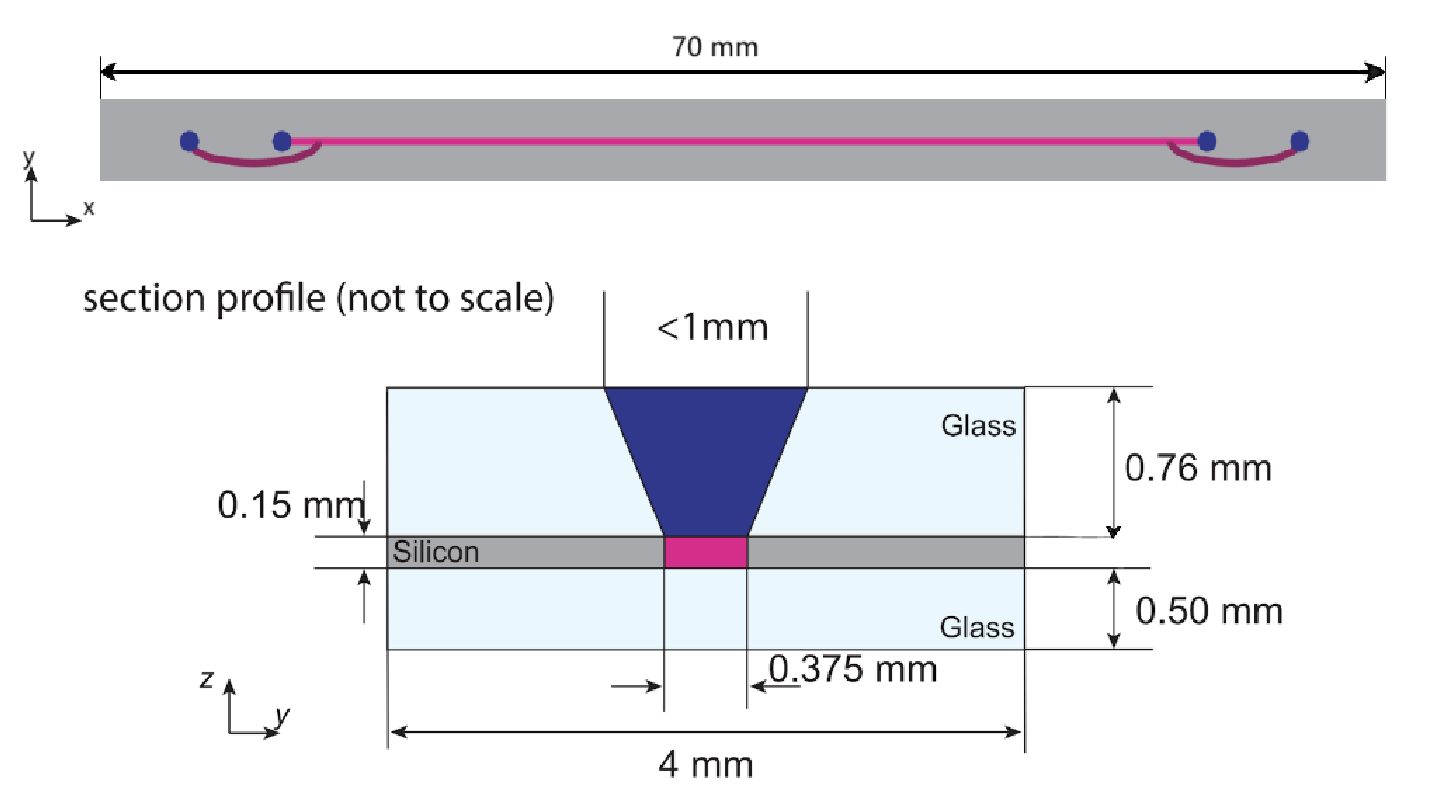
\includegraphics[width=7.5cm]{Images/Updated_figure1.png} %figurer sparas lämpligen i eps format
\caption{Dimensions of the microchip and of the cross section where the light blue is glass, gray is the silicon chip and the dark blue is the inlet of the channel and magenta is the channel itself. }
\label{DimensionMicrochip}
\end{center}
\end{figure} % Micro chip dimensions 1

which sat on a microscope (Olympus BX51WI). On the side, a 2MHz piezo element, and on the bottom of the microchip a 5MHz piezo element (Lead zirconate titanate (PZT) transducers, Pz26, Ferroperm Piezoceramics, Kvistgaard, Denmark) were glued on (Loctite Super Glue, Henkel Norden AB, Stockholm, Sweden) with a thickness-mode actuation frequency of 2MHz and 5MHz respectively. Both the beginning and end of the channel had a central and side inlet, connected to tubing (made of PTFE, inner diameter 0.3 mm, outer diameter 1.6 mm). The two inlets delivered the two liquids for mixing. One, none or both of the liquids may be heated by a large container with hot water (Grant GD100 Heat Bath) or cooled to zero degrees with an ice bath (home made Styrofoam container), depending on the experiment. The liquids were both injected with infusion pumps (WPI KDS-210-CE Infusion Pump), which used 10 ml syringes. The outlets lead the liquids to a waste container.  

For a liquid to be heated by the bath, it would have to be stored in a container under water, while also being able to be propelled by the syringe pump. The solution for this problem was taken by F.Burgoyne \cite{Burgoyne} which make use of two syringes tail to tail, held together by a clamp (KECK CG-145 Clamp). When one of the syringes would fill up, the other one would empty and the contraption could then both store the liquid under water and move.

\begin{figure}[h]
\begin{center}
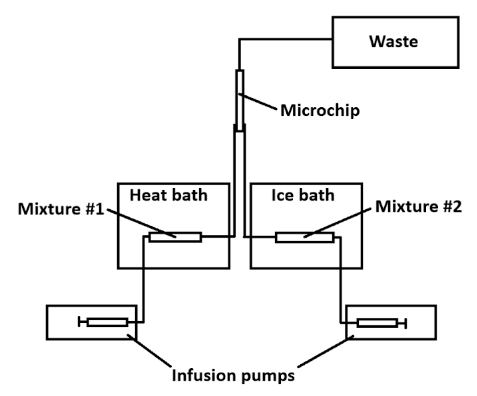
\includegraphics[width=8.5cm]{Images/ExperimentSetUp.png} %figurer sparas lämpligen i eps format
\caption{The overarching experimental setup where the heat and ice baths may be excluded depending on the sub-experiment.}
\label{Setup}
\end{center}
\end{figure} % Experimental setup 2

The function generator (Tektronix AFG 3022B Dual Channel Arbitrary/Function Generator) was connected to the piezo elements with coaxial cables. The generator excites the elements electrically which in turn vibrate the micro channel and excite the mechanical resonance. The function generator could only output $10 V_{pp}$ so an amplifier (home made amplifier) was used to boost the voltage to about $30 V_{pp}$. An oscilloscope (Tektronix TBS1052C Digital Oscilloscope) was also used to more accurately measure the voltage as well as to make sure the sinusoid was not distorted by the amplification.

To capture the images, a camera (Hamamatsu Digital Camera C13440-ORCA-flash4.0) was used which connected to a computer where it was processed by ImageJ (version 1.51s). Some of the liquids required a specific wavelength to fluoresce and a lumination system (CoolLED pE-4000) was used to excite the specific wavelength of light. 




\subsection{Calibrating actuation frequency of 2MHz and 5MHz piezo-element}
To determine the best actuation frequency for each piezo element, particles (5$\mu$m diameter, Fluoro-Max, Thermo Fisher Scientific, Waltham, Massachusetts) were used to visualize the standing wave in the liquid. 

For the 2MHz element a first order harmonic standing wave should generate a pressure node in the middle of the channel (Figure \ref{2vs5Actuation}). Particles were injected with a rate of 100$\mu$L/min and pictures were taken 100 at a time at an interval of 10 ms. The images were eventually averaged to visualize the flow patterns of the particles.

At first the calibration started at 2MHz and measurements in steps of 0.1MHz was made until a satisfactory image was made. More fine tuning into steps of 0.01MHz was done by calculating the full width at half maximimum (FWHM) value, assuming that the particles would flow in a Gaussian distribution. This was done by putting all the points which have a normalized value above 0.5 in a vector and then calculating the length of the vector to get the FWHM where a lower value would mean a sharper peak. This process repeated into lower decimals until no significant changes was visible.

When calibrating the 5MHz element, a different approach had to be made. The microscope observes the channel on the horizontal plane, while the standing wave is generated vertically. 

\begin{figure}[h]
\begin{center}
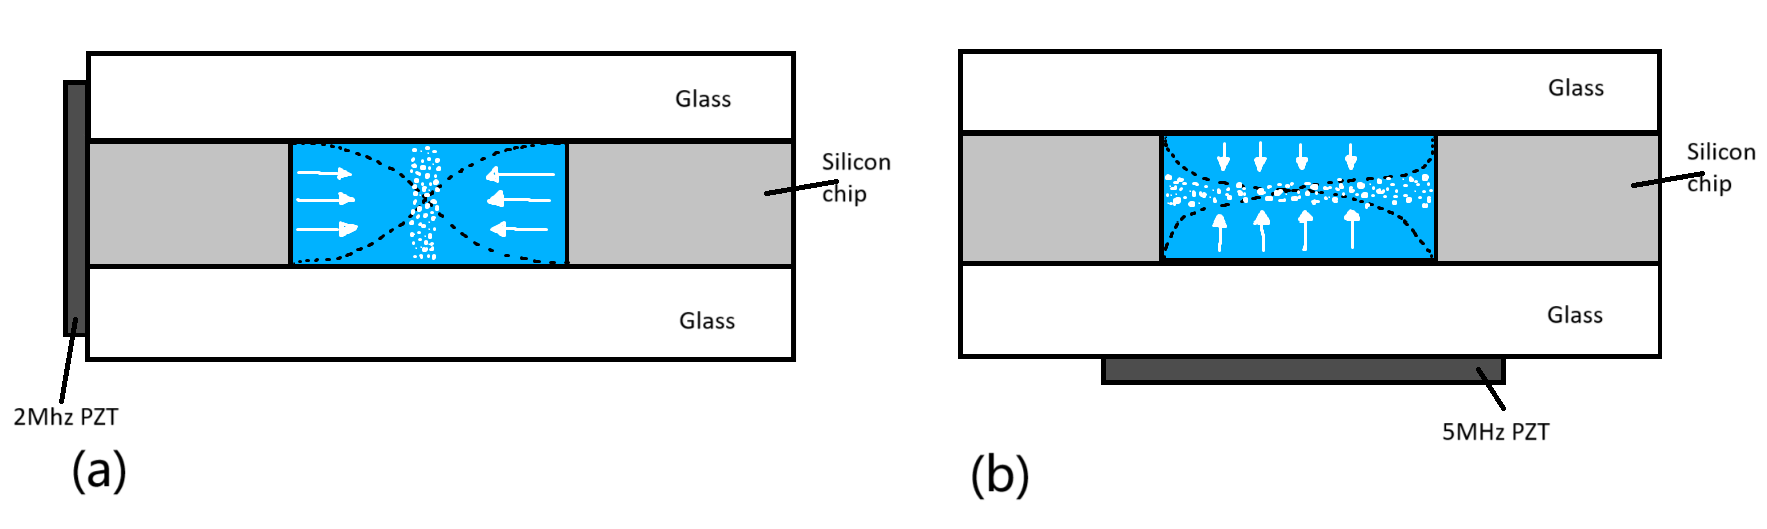
\includegraphics[width=8.7cm]{Images/2and5_in_one(final).png} %figurer sparas lämpligen i eps format
\caption{Channel cross section of 2MHz standing wave actuation (a) vs 5MHz standing wave actuation (b), where the images are taken from a camera above.}
\label{2vs5Actuation}
\end{center}
\end{figure} % Ossian drawn image 3

A stop flow observation was made instead, where particles were introduced into the system and then sedimented to the bottom. When a standing wave is actuated, particles will move vertically to the position of the pressure node (Figure \ref{2vs5Actuation}). Ideally a standing wave of the first harmonic order will result in a pressure node halfway in height of the channel. To confirm a correctly actuated frequency, the microscope is tuned to let anything moving in half the height to come into focus. 100 pictures were taken at an interval of 10ms, and during the acquisition process the signal generator was activated. The images were then analyzed to see how many particles that came into focus during the acquisition process.

\subsection{Relationship between temperature and intensity with the use of Rhodamine in heat bath}

First, a standardized background image was taken of the channel with MilliQ (distilled water) flowing through. Rhodamine B (RhB)  (40$\mu$M) was afterwards heated up with the heat bath and then was injected into the channel at a rate of 100$\mu$L/min and was let to stabilize. To determine stabilizations, pictures were taken continuously and when the intensity no longer shifted, 100 images were taken with a 10ms interval. The temperature was increased and this process was repeated.

\subsection{Relationship between temperature and intensity with the use of rhodamine in ice bath}

First, a standardized background image was taken of the channel with MilliQ flowing through. Rhodamine (40$\mu$M) was afterwards cooled down with the ice bath with a temperature of zero degrees, and was then injected into the channel with a rate of 100$\mu$L/min and was let to stabilize. To determine stabilizations, pictures were taken continuously and when the intensity no longer shifted, 100 images were taken with a 10ms interval. Only one measurement was made compared to the heat bath analysis, considering that controlling the temperature of the ice bath is not possible at the time.

\subsection{Temperature loss in tubing}

A standardized background image was taken with MilliQ flowing through. Rhodamine (40$\mu$M) was afterwards heated up with the heat bath to 60 degrees and 165cm tubing connecting the rhodamine in the heat bath to the microchip was exposed to the environment. Rhodamine was then injected into the channel at 50$\mu$L/min and pictures were taken to determine stabilized flow. 100 images at 10ms intervals were taken at the input of the micro channel as measurements. Parts of the tubing were then put in the heat bath, lowering the distance in which the tubing was exposed to the environment, and this process was repeated.

\subsection{Temperature generated by the 2MHz and 5MHz element}
\label{tempelements}

Even though there is a heat and ice bath to generate the temperature gradient, the PZT's can also act as heat source by dissipating electrical energy when converting it into mechanical vibration, hence generating heat. In order to specify if mixing efficiency is due to the temperature gradient generated by external sources or piezo related sources, experiments were conducted to specify the capabilities in the elements as a heat source. Rhodamine was injected into the channel at a rate of 100$\mu$L/min and at first a voltage of 0 volts was applied to the element to be investigated. 100 pictures were taken at an interval of 10ms, and afterwards the voltage was increased by 2.5 volts. This process was repeated up to 30 volts and the experiments were done with the 2MHz and 5MHz element separately with their respective resonance frequency.

\subsection{Finding the optimal setup}

In order to perform a parameter analysis, the most efficient setup had to be found. This would then become the standard point to compare to during the analysis. At first, different combinations where used with the piezo elements: 2MHz PZT alone, 5MHz PZT alone 2MHz and 5MHz PZT’s at the same time. The capabilities of the function generator was maximized to observe the maximum mixing effects that could be achieved.

\subsection{Parameter analysis}

When using \textit{temperature} as a parameter, the 2MHz PZT was used as the actuation source, Rhodamine (40$\mu$M) and MilliQ was placed in the heat bath at initially 20 degrees. Fluorescein (30$\mu$M) was placed in room temperature (around 20 degrees). Throughout the experiment, an injection speed of 50$\mu$L/min was used for all measurements. Fluorescein (in room temperature) and MilliQ (in heat bath) was injected into the channel, and sound was activated. 100 images were taken at 10ms interval, measuring the mixing effect at this temperature difference. Rhodamine (in heat bath) was then injected by itself into the channel to measure the temperature intensity during the mixing measurement. Temperature of the heat bath was increased, and this process was repeated.

When the heat bath reached 60 degrees, the temperature was reset down to 20 degrees, and the experiment continued but with the ice bath in play. The fluorescein (30$\mu$M) that was initially placed at room temperature, was here on placed in the ice bath, cooling it down to an estimated temperature of zero degrees. A new mixture of Rhodamine was placed in the ice bath to also cool down to zero degrees. Rhodamine was afterwards injected by itself into the channel to measure the temperature intensity given by the ice bath. MilliQ (in the heat bath) and fluorescein (in the ice bath) was injected in the channel, and 100 images were taken at an interval of 10ms to measure mixing effects at this temperature difference. No more rhodamine measurements from the heat bath were taken during this phase of the experiment, considering that they were already taken before. Temperature of the heat bath was increased, and this process repeated.

When using \textit{voltage} as a parameter, the 2MHz PZT was used as the actuation source, MilliQ was put in the heat bath and set to 60 degrees and the fluorescein (30$\mu$M) in the ice bath, cooled down to a temperature of zero degrees. Fluorescein and MilliQ was injected into the channel at 50$\mu$L/min, and actuation started initially at $0 V_{pp}$. 100 images were taken at an interval of 10ms for measurements. Voltage was increased, and the process was repeated. 

When using \textit{flow ratio} as a parameter, the 2MHz PZT was used as the actuation source, MilliQ was put in the heat bath which was set to 60 degrees and fluorescein (30$\mu$M) in the ice bath, cooled down to a temperature of zero degrees. Fluorescein and MilliQ was injected into the channel at initially 50$\mu$L/min. Sound was activated, and 100 images were taken at 10ms interval for measurements. The flow rate was then increased for MilliQ, changing the ratio of MilliQ and fluorescein flowing through the channel. Measuring images were taken again, and this process was repeated.

During this part of the project, input parameters were assumed to be independent of each other, hence the analysis being performed with only one changing variable between measurements.

\subsection{Calculating intensities}
\label{CAI}

After measurements had been made, the images were further processed in MATLAB for analysis. The general idea was that by taking 100 images at a time for one data point and afterwards creating an image that represents the average of these images, errors would be less significant and a representative image could be analysed for that particular instance. Figure \ref{2MHzComparison} is an example of images that were generated by taking the average of 100 images. To further process intensities, the mean intensities in the axial direction were taken as a function of channel width. Figure \ref{codeexample} shows how the intensity data was generated. Plotting the values generated from the code in Figure \ref{codeexample} when using image (b) shown in Figure \ref{2MHzComparison} generates the graph shown in Figure \ref{example}.

\begin{figure}[H]
\begin{center}
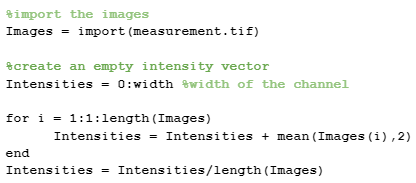
\includegraphics[width=7cm]{Images/code example.png} %figurer sparas lämpligen i eps format
\caption{Example code in MATLAB that generates the mean intensity of the channel as a function of channel width. Be aware that this code is purely representative of the general calculations to give an idea of how images were processed.}
\label{codeexample}
\end{center}
\end{figure} % Code 4

\begin{figure}[H]
\begin{center}
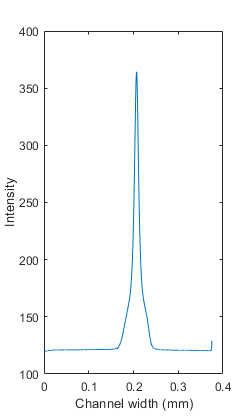
\includegraphics[width=3.7cm]{Images/example.png} %figurer sparas lämpligen i eps format
\caption{Intensity as a function of channel width, based on image (b) in Figure \ref{2MHzComparison}.}
\label{example}
\end{center}
\end{figure} % Graph example 5

\subsection{Quantifying mixing}
\label{CAQ}

When quantifying mixing, refer to Figure \ref{mixing calc example} as an example. The figure is a measurement taken during parameter analysis, white color is fluorescein and black is MilliQ. Looking at the graph, one can see that the intensity of MilliQ is 3.7\% of the intensity emitted by fluorescein. If complete mixing would occur, the intensity of MilliQ would be close to 100\%. So for this measurement, \textit{mixing} is approximately 3.7\%. During the parameter analysis, this was the method used to quantify \textit{mixing}.

\begin{figure}[H]
\begin{center}
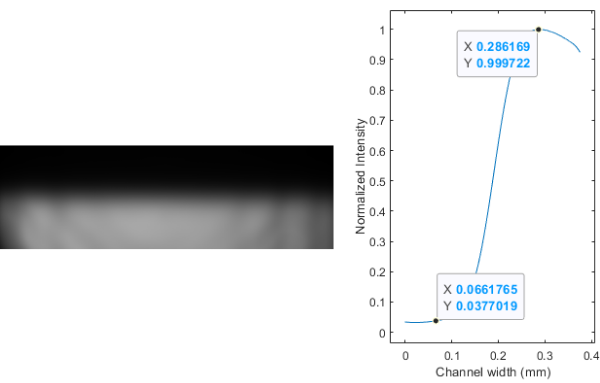
\includegraphics[width=7.5cm]{Images/mixing calc example.png} %figurer sparas lämpligen i eps format
\caption{Intensity as a function of channel width, with its corresponding averaged image. White is fluorescein and black is MilliQ.}
\label{mixing calc example}
\end{center}
\end{figure} % Image and Graph 6



%--------------------------------------------------------------------------------------------------------------------------------------------------

\section{Results} 

\subsection{Calibrating resonance frequency of 2MHz and 5MHz piezo-element}
Finding the actuation frequency for the half-standing wave resonance in the channel width (theoretical 2MHz) involved tweaking the frequency and calculating the full width half maximum (FWHM). The resulting frequency which had the lowest (and thereby most focused) FWHM was \textit{1.9164 MHz}. Figure \ref{2MHzComparison} shows a comparison between 1.8 MHz and the final frequency of 1.9164 MHz. 

\begin{figure}[!htb]
\begin{center}
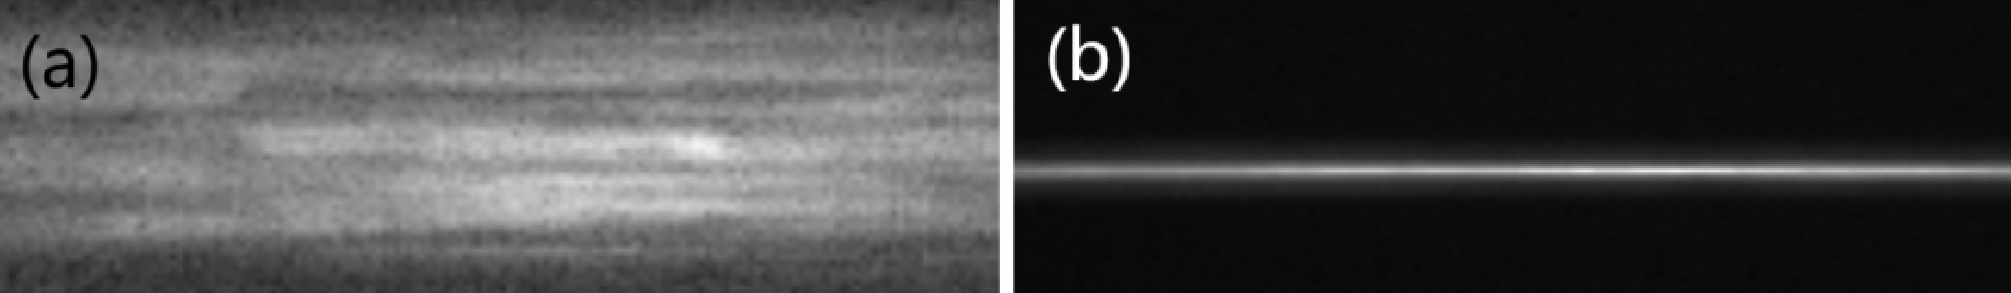
\includegraphics[width=8.7cm]{Images/2MHz_actuation.png} %figurer sparas lämpligen i eps format
\caption{An example of a poorly calibrated frequency (a) where the FWHM is 648 pixels, and a correctly calibrated one (b) where the FWHM is 87 pixels.}
\label{2MHzComparison}
\end{center}
\end{figure} %2MHz actuation 7

At first the calibration started at 5MHz and repeated in steps of 0.1 MHz and lower until a satisfactory image was obtained. The method for quantifying the best frequency was done through visual measurement when the particles were in focus. From the images taken it was determined that \textit{4.775MHz} gave the best result. Figure \ref{5MHzComparison} shows clearly that when the PZT was resonating, the particles were significantly more in focus. Using a more numerical approach such as 3D particle tracking based on in and out of focus diffraction \cite{Tasadduq} would result in improved precision, but is more time consuming and outside the scope of the thesis work.


\begin{figure}[H]
\begin{center}
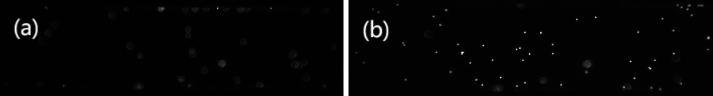
\includegraphics[width=8.7cm]{Images/5mhz_actuation.png} %figurer sparas lämpligen i eps format
\caption{The focus of the camera is in the middle plane of the channel. Image (a) shows the channel when the function generator is off and thereby the particles are at the bottom and not in focus. Image (b) has the function generator on and the particles have moved into focus at the 5MHz PZT's actuation frequency.}
\label{5MHzComparison}
\end{center}
\end{figure} %5Mhz actuation 8

\subsection{Efficiency analysis}
\label{efficiencyanalysis}

RhB generates intensities that get stronger in lower temperatures and weaker in higher temperatures. Thus, temperature loss in the analysis is shown as an increase in intensity. In this project, RhB intensities is also assumed to be linear with temperature \cite{Corato}. A decrease by a certain percentage in intensity is assumed to be linear in change  in absolute temperature.

Thermal properties of the components involved were analyzed. In section \ref{tempelements} it was stated that the PZT's are prone to heat generation as voltage increases. By analyzing the capabilities of the PZT's as a heat source, its acoustic capabilities can be separated from its thermal capabilities. Figures \ref{2MHzHeat} and \ref{5MHzHeat} show the intensity differences at different voltages, normalized according to the intensity generated at $0 V_{pp}$.

\begin{figure}[H]
\begin{center}
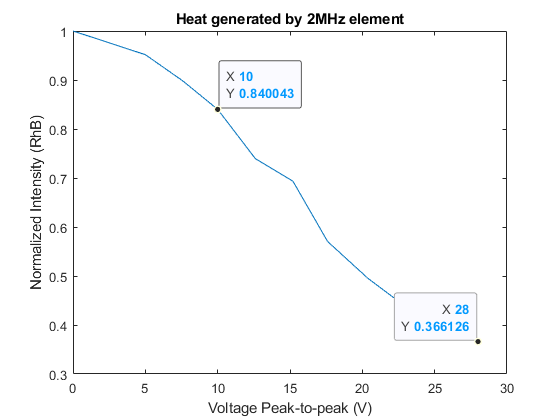
\includegraphics[width=7cm]{Images/Images from Jonte/heat generated by 2mhz element.png} %figurer sparas lämpligen i eps format
\caption{RhB intensity differences at different voltages.}
\label{2MHzHeat}
\end{center}
\end{figure} %Heat from 2mhz element 9

\begin{figure}[H]
\begin{center}
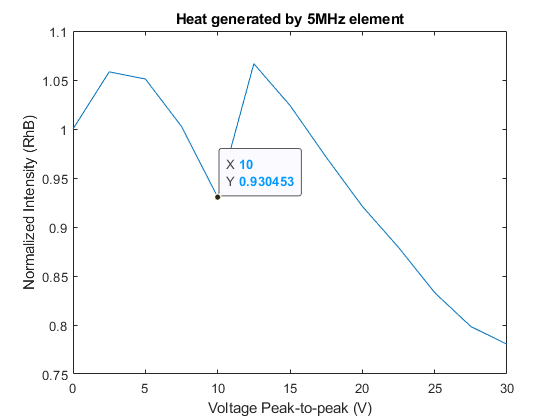
\includegraphics[width=7cm]{Images/Images from Jonte/heat generated by 5mhz element.png} %figurer sparas lämpligen i eps format
\caption{RhB intensity differences at different voltages. $10 V_{pp}$ is marked to compare to the efficiency of the 2MHz PZT. The jump in voltage at around $12 V_{pp}$ is due to a refill of RhB in the syringes, which may have differed slightly in concentration.}
\label{5MHzHeat}
\end{center}
\end{figure} %Heat from 5mhz element 10

With the data stating the thermal aspects of the PZT's ready, more analysis was done on the heat and ice baths. Similarly to Figures \ref{2MHzHeat} and \ref{5MHzHeat}, mean intensities of RhB was analyzed, where the normalization is done in regards to the mean intensity generated at room temperature.

\begin{figure}[H]
\begin{center}
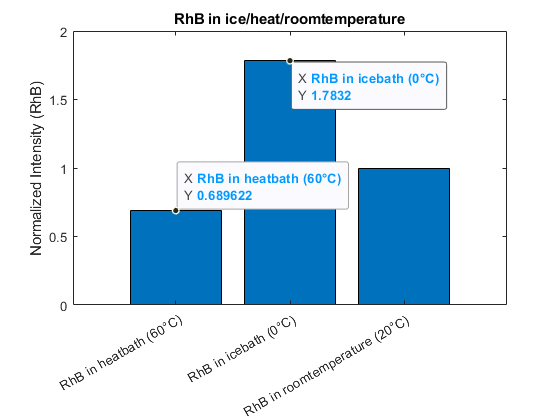
\includegraphics[width=7cm]{Images/Images from Jonte/RhD in ice.heat,roomtemperature.png} %figurer sparas lämpligen i eps format
\caption{Heat generated by respective bath compared to room temperature.}
\label{RhDIceHeatRoom}
\end{center}
\end{figure} %RhB in ice/heat/room 11

Lastly, thermal loss in tubing was analyzed. Analysis started with 0\% of tubing submerged in the heat bath and sections were successively added. The intensities during each measurement is shown in Figure \ref{Tubing} as normalized according to the mean intensity during the 0\% submerge.

\begin{figure}[H]
\begin{center}
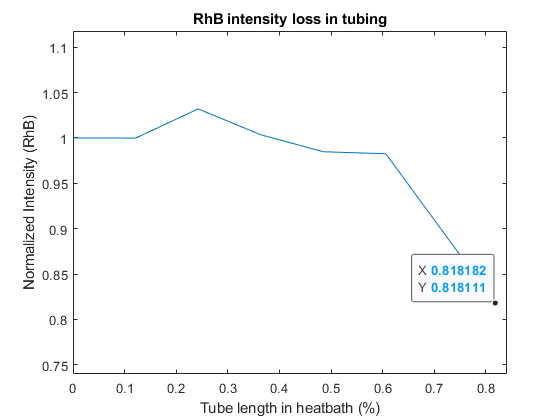
\includegraphics[width=7cm]{Images/Images from Jonte/rhd intensity loss in tubing.png} %figurer sparas lämpligen i eps format
\caption{Normalized intensity as a function of the proportion of tubing submerged in the heatbath}
\label{Tubing}
\end{center}
\end{figure} %Tubing 12

In Figures \ref{2MHzHeat}, \ref{5MHzHeat} and \ref{RhDIceHeatRoom}, normalization was done according to room temperature. At $0 V_{pp}$ in Figures \ref{2MHzHeat} and \ref{5MHzHeat}, the temperature of the RhB is room temperature. Therefore the figures mentioned can be compared accordingly to make a judgement of thermal aspects. Figure \ref{Tubing} on the other hand is not normalized to an intensity in room temperature. This figure is solely to give an estimate of thermal retention.

An example of an analysis using these results; the gradient created by the heat and ice bath can be estimated to follow characteristics of Figures \ref{RhDIceHeatRoom}, but only a certain percentage of that gradient will be preserved based on the tubing in Figure \ref{Tubing}, and adding to that gradient, the PZT's will contribute with heat according to Figures \ref{2MHzHeat} and \ref{5MHzHeat}.

\subsection{Finding the optimal setup}

\begin{figure}[H]
\begin{center}
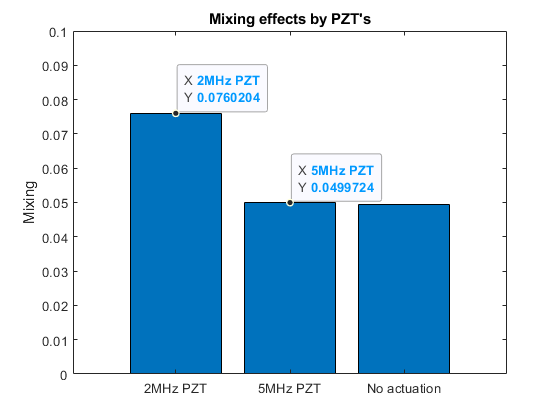
\includegraphics[width=7cm]{Images/Images from Jonte/Mixing effects by PZT_s.png} %figurer sparas lämpligen i eps format
\caption{Mixing was calculated as per calculations mentioned in section \ref{CAQ}.}
\label{PZT}
\end{center}
\end{figure} % Mixing (2mhz and 5mhz)  13

Judging from the results in Figure \ref{PZT}, the analysis of mixing effects when combining the 2MHz PZT and 5MHz PZT was skipped due to no significant effects in mixing when using the 5MHz PZT alone.

\subsection{Parameter analysis}

\begin{figure}[H]
\begin{center}
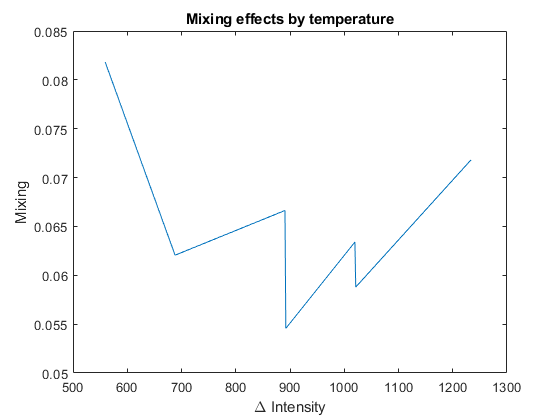
\includegraphics[width=8cm]{Images/Images from Jonte/Mixing effects by temperature.png} %figurer sparas lämpligen i eps format
\caption{Mixing as a function of \(\Delta\)intensity.}
\label{Temperature}
\end{center}
\end{figure} % Mixing Temperature 14

Because of thermal retention problems according to section \ref{efficiencyanalysis}, presenting quantified mixing as a function of absolute \(\Delta\)T would be incorrect. During measurements, intensities of RhB was taken as \(\Delta\)T increased. Instead of presenting the data as a function of \(\Delta\)T, \(\Delta\)intensity was used instead. RhB can be assumed to be proportional in intensity to its temperature, therefore this comparison can be made instead. \cite{Corato}

\begin{figure}[H]
\begin{center}
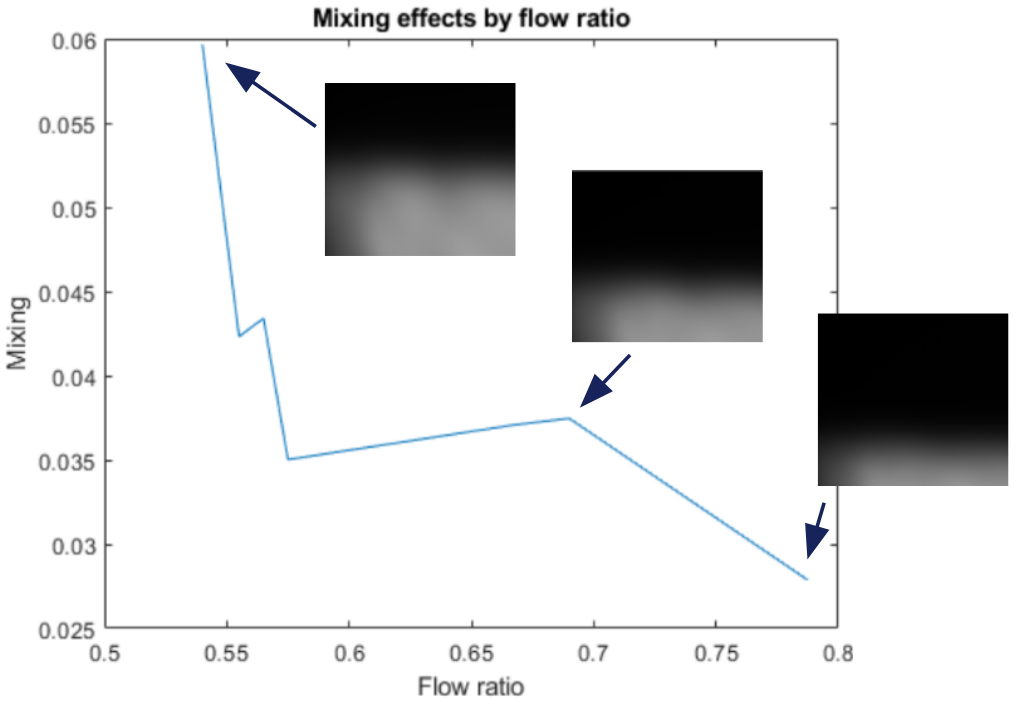
\includegraphics[width=7.9cm]{Images/Images from Jonte/Mixing effects by flow ratio.png} %figurer sparas lämpligen i eps format
\caption{Mixing as a function of flow ratio. Flow ratio is the \% distribution between MilliQ and Fluorescein in the channel. 0.5 corresponds to 50\% of MilliQ and 50\% of fluorescein, and 0.7 corresponds to 70\% MilliQ and 30\% Fluorescein.}
\label{FlowRatio}
\end{center}
\end{figure} % Mixing Flow rate 15

\begin{figure}[H]
\begin{center}
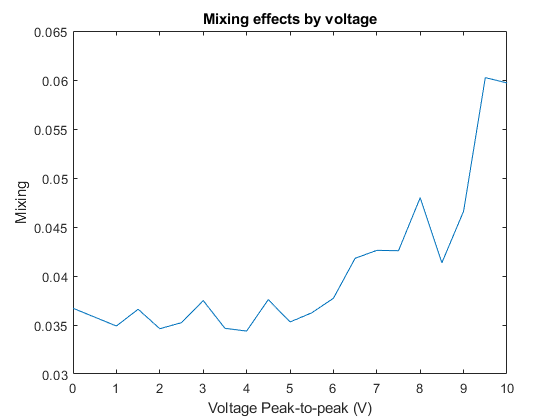
\includegraphics[width=7.9cm]{Images/Images from Jonte/Mixing effects by voltage.png} %figurer sparas lämpligen i eps format
\caption{Mixing as a function of voltage (2MHz PZT)}
\label{Voltage}
\end{center}
\end{figure} % Mixing Voltage 16
%\FloatBarrier

%--------------------------------------------------------------------------------------------------------------------------------------------------

\section{Discussion}

\subsection{Efficiency analysis}

When analyzing the data, one contradictory conclusion can be made. In Figure \ref{RhDIceHeatRoom} there is a noticeable difference in temperature retention between the ice bath and the heat bath, where the ice bath contributes to a difference of 78\%  in RhB intensity compared to the heat bath that reduces intensity by 31\%.

This is unexpected since the ice bath had a temperature difference of 20 degrees while the heat bath had a temperature difference of 40 degrees. Still, using the ice bath resulted in a much larger intensity difference than using the heat bath.  

Some potential reasons were derived post-measurement. Throughout measurements the temperature of the heat bath was increased over time and due to the dimensions of the heat bath, a notable amount of heat was dissipated into the environment. Higher temperatures in the heat bath lead to increased dissipation, which lead to higher room temperatures. What was estimated to be room temperature at the start of the experiment could differ greatly from the room temperature at the end of the experiment. The ice bath consisted of an insulated container made of Styrofoam, therefore it was safe to assume that dissipation from the container would be insignificant. When comparing the intensities of the heated/cooled liquids with the room temperature at the time, the \% difference would differ greatly.

Another potential reason is the tubing. The micro environment and tubing used increased thermal diffusion compared to its macro counterpart. The thinness and narrow diameter of tubing resulted in the results shown in Figure \ref{Tubing}. Exposing more parts of the tubing led to temperature loss to an estimated 18\%. Dissipation through the tubing is a function of temperature differences between liquid and environment, which can also explain the improved retention performance by the ice bath, considering that the temperature difference is 20 degrees compared to 40 degrees in the heat bath.

Lastly, the liquid to be heated was placed far away from the heating coils in the heat bath. This could have led to misleading temperatures in the liquids, as the temperature reader showed one temperature, but could be far colder away from the reader.

These results are of significant importance considering that mixing analysis in later parts of the project relied on inhomogeneity in temperatures. These errors are noticeable in Figure \ref{Temperature} with oscillating data points, where the temperatures differences were in parts generated by the ice bath and room temperature. Because of the inconsistencies in room temperatures, temperature differences during those measurements might not have been accurate. Another possible reason could be the fact that RhB is roughly linear but the estimation begins to falter when temperatures approach 0 degrees\cite{Natrajan}.

\subsection{Finding the optimal setup}

When finding the optimal setup, Figure \ref{PZT} shows that the 5MHz PZT made no difference in mixing potential. Published literature in the same field suggests the opposite of the observed results \cite{Corato}. 

The conclusion from the analysis was that unfortunately, the 5MHz PZT was not effective in this setup. For this reason, the parameter analysis continued with only the 2MHz PZT.

\subsection{Parameter analysis}

There is a noticeable correlation between mixing efficiency and voltage, as shown in Figure \ref{Voltage}. The exponential increase may be partly due to the increased heat dissipation by the PZT as voltage increases. As both the acoustic energy and thermal gradient increases, it is difficult to decouple the combined effects and understand which part of mixing efficiency is due to the increase in acoustic field or increase in thermal gradient.

In Figure \ref{Voltage} the voltages in the parameter analysis ranged from $0 V_{pp}$ to $10 V_{pp}$, while in Figure \ref{2MHzHeat} and \ref{5MHzHeat} the voltages ranged from $0 V_{pp}$ up to $30 V_{pp}$. The reason behind the difference in voltages was due to the amplifier being broken at the time of the analysis.

As per the reason stated during the efficiency analysis, the temperature parameter oscillates considerably and is difficult to analyse. This oscillation may be due to the thermal aspects during the efficiency analysis, or due to mixing not having a significant effect, but it is difficult to say.

Regarding the flow ratio, there is a significant drop in the mixing efficiency as the interface moves away from the pressure node, as shown in Figure \ref{FlowRatio}. However, there is a window in the data points where an interval of ratios are missing. Between 57\% and 78\% flow ratio there exists only one measurement, therefore it is difficult to discern the complete behavior behind mixing and fluid distribution. Identifying a linear/non-linear relationship is hard to derive for this reason, but according to data available, results show that mixing is best at 50\%/50\% ratio of distribution of fluids.

In this project the heat and ice bath is an example of an external heating method. Besides the usage of generating a thermal gradient, one other aspect needs to be brought to attention. One advantage of utilizing internal heating instead of external heating is the usage of thermal convection to contribute to flows \cite{Corato}. Convection arises from temperature differences between fluids. In our setup, throughout the channel as mixing occurs the thermal inhomogeneity gets weaker due to thermal diffusion and therefore less convection is involved. Internal heating methods ensures continuous thermal inhomogeneity and thus allows the acoustic field to influence mixing to greater extents.

\subsection{Ethics and sustainable development}

Innovation is sometimes in a heated battle between ethics and sustainable development. It is weighing the improvement of human life versus strain on the environment. Our method has applications such as mixing in lab-on-a-chip systems which is the future of medicine, especially for those people in need. The vision is for it to be a cheap way to democratize healthcare for all. Mixing in microfluidic devices is a huge problem for these applications and this is a direct response to that outcry.

The methods used in the laboration all depend on using a temperature difference and therefore needs an external heat source. Also, ultrasound is used, and thus a function generator or something similar is also needed. Current solutions rely on passive diffusion which obviously has less power consumption than our method, though the mixing is heavily compromised \cite{Qiu}. 

The amount of energy consumption the method requires is made up of the energy it takes to heat the water and the energy it takes to actuate the ultrasound field. If it is assumed that 10ml  water (which is quite a large amount in microfluidics) needs to be heated up from room temperature to 60 degrees Celsius, then using the heat capacity of water, it would take 167 Joules to be heated. This amount of energy is negligible. The function generator used (Tektronix AFG 3022B) has a data sheet \cite{Datasheet} which states that the power consumption for any setting is less than 120 W, which is not negligible but still a small amount of energy consumed for each experiment since it is only active for a minute maximum.

The materials used for the microchip are primarily pyrex glass and silicon. Neither of these materials are biodegradable and are a crutch on the method’s sustainability \cite{Graiver, Adekomaya}. Though, the dimensions of the chip is only 70mm x 4mm x 1.4mm so the total amount of material used is extremely small. Also, the chip can be used multiple times for years if handled properly.

\subsection{Outlook on decisions}
If we would have done the project again with hindsight, we would make sure that the room temperature was not assumed to be constant, especially with a heat bath in the room. Also, having a much greater insulation on the tubing would lead to an decrease in heat loss which was one of the main problems throughout the experiments. Another mistake was the mixing of rhodamine and fluorescein concentrations, which we afterwards realized varied throughout some measurements. 




%--------------------------------------------------------------------------------------------------------------------------------------------------

\section{Conclusion}
The conclusion of this project states that thermoacoustic mixing relies heavily on the acoustic field. More acoustic energy deposited into the liquids may affect mixing to greater extents than the thermal gradient does, however the setup that was used to generate the thermal gradient had errors in retention. Moving the interface of the liquids outside the pressure node leads to weaker performance, and therefore it is advisable to retain a 50\% vs 50\% distribution.

%--------------------------------------------------------------------------------------------------------------------------------------------------

\section{Acknowledgements}

We would like to thank our supervisor Enrico Corato at the biomedical engineering department of LTH, for giving us the opportunity to partake in our first big project as future engineers. Thank you for providing us with the tools and helping us whenever we felt lost.
 
%--------------------------------------------------------------------------------------------------------------------------------------------------




%--------------------------------------------------------------------------------------------------------------------------------------------------

\newpage
\begin{thebibliography}{99} % IEEE-format

\bibitem{Bruus} Bruus, H. (1997) ‘Basic concepts in Microfluidics’, \textit{Theoretical Microfluidics}, pp. 1–18.

\bibitem{Deshmukh} Deshmukh, S. et al. (2014) ‘Acoustic radiation forces at liquid interfaces impact the performance of acoustophoresis’, \textit{Lab Chip}, 14(17), pp. 3394–3400. 

\bibitem{Jonas} Jonas, T. Qiu, W. Augustsson, P. Bruus, H. (2018) ‘Acoustic streaming and its suppression in inhomogeneous fluids,’, \textit{Phys. Rev. Lett}.

\bibitem{Jonastensor} Jonas, T. Augustsson, P. Bruus, H. (2016) ‘Acoustic force density acting on inhomogeneous Fluids in acoustic fields,’, \textit{Phys. Rev. Lett}.

\bibitem{Sharda} Gupta, S. Bit, A. (2019) ‘Acoustophoresis-based biomedical device applications’, \textit{Science Direct}. 

\bibitem{Laurell} Laurell, T., Petersson, F. and Nilsson, A. (2007) ‘Chip integrated strategies for acoustic separation and manipulation of cells and particles’, \textit{Chem. Soc. Rev}, 36(3), pp. 492–506.

\bibitem{Mitome} Mitome, H. (1998) ‘The mechanism of generation of acoustic streaming’, \textit{Electronics and Communications in Japan (Part III: Fundamental Electronic Science)} 81(10), pp. 1–8.

\bibitem{Corato} Corato, E. (2020) ‘Thermal Acoustic Flow inside an Ultrasound Resonator‘. Master’s thesis. Department of Biomedical Engineering.

\bibitem{Qiu} Qiu, W. et al. (2021) ‘Fast microscale acoustic streaming driven by a temperature-gradient-induced nondissipative acoustic body force’, \textit{Physical Review Letters}, 127(6). 


\bibitem{Ward} Ward, K. and Fan, Z.H. (2015) ‘Mixing in microfluidic devices and enhancement methods’, \textit{Journal of Micromechanics and Microengineering}, 25(9). 


\bibitem{Burgoyne} Burgoyne, F. (2008) An easy temperature control system for syringe pumps, Royal Society of Chemistry. Available at: 

\url{https://blogs.rsc.org/chipsandtips/2008/04/22/an-easy-temperature-control-system-for-syringe-pumps/?doing_wp_cron=1706726295.3376879692077636718750} (Accessed: 08 May 2024)

\bibitem{Natrajan} Natrajan, V.K. and Christensen, K.T. (2008) ‘Fluorescent thermometry’, \textit{Encyclopedia of Microfluidics and Nanofluidics}, pp. 750–759. 

\bibitem{Tasadduq} Tasadduq, B. et al. (2015) ‘Three-dimensional particle tracking in microfluidic channel flow using in and out of Focus Diffraction’, \textit{Flow Measurement and Instrumentation}, 45, pp. 218–224. 

\bibitem{Datasheet} ‘Arbitrary/Function Generators - AFG3000 Series’ [Datasheet], \textit{Tektronix}, (Published: 27 Jul 2012)


\bibitem{Graiver} Graiver, D., Farminer, K.W. and Narayan, R. (2003) ‘A Review of the Fate and Effects of Silicones in the Environment’, \textit{Journal of Polymers and the Environment}, 11(4), pp. 129–136. 

\bibitem{Adekomaya} Adekomaya, O. and Majozi, T. (2021) ‘Mitigating environmental impact of waste glass materials: Review of the existing reclamation options and future outlook’, \textit{Environmental Science and Pollution Research}, 28(9), pp. 10488–10502.



\end{thebibliography}

\end{document}